% ----- formatovani dokumentu -----------------------------------------------
\documentclass[12pt,a4paper,titlepage,final,tikz,border=4mm]{report}
\usepackage[utf8]{inputenc}
\usepackage{times}
\usepackage[T1, IL2]{fontenc}
\usepackage{graphicx}
\usepackage{subcaption}
\usepackage{epstopdf}
\usepackage[margin=2cm]{caption}
\usepackage[top=3cm, left=2cm, right=2cm, text={17cm, 24cm}, ignorefoot]{geometry}
\usepackage{color}
\usepackage{url}
\usepackage{setspace}
\usepackage{listings}
\singlespacing
\usepackage[square, numbers]{natbib} 
\pagestyle{plain}
\pagenumbering{arabic}
\setcounter{page}{1}
\usepackage{amsmath}
\setcounter{secnumdepth}{-1}
\setlength{\parindent}{1cm}	
\usepackage{natbib}
\usepackage{listings}
\usepackage[linguistics]{forest}
\usepackage{minted}
\usetikzlibrary{positioning,fit,calc}
\tikzset{block/.style={draw,thick,text width=2cm,minimum height=1cm,align=center},line/.style={-latex}}
% ----- vyberte jazyk -------------------------------------------------------
\usepackage[czech]{babel}
%\usepackage[english]{babel}

% ----- dopiste titulky -----------------------------------------------------
\newcommand\Course{Visualization \& CAD}
\newcommand\WorkTitle{Animation of the procession of penitents among penitents}
\newcommand\AuthorB{Patrik Chukir}
\newcommand\AuthorBEmail{xchuki00@stud.fit.vutbr.cz}
\newcommand\Faculty{Faculty of Information Technology}
\newcommand\School{Brno University of Technology}

\usepackage[
pdftitle={\WorkTitle},
pdfauthor={\AuthorB},
bookmarks=true,
colorlinks=false,
breaklinks=true,
urlcolor=black,
citecolor=black,
linkcolor=black,
unicode=true,
]
{hyperref}


% ----- titulni strana ------------------------------------------------------

\begin{document}
	\begin{titlepage}
	\begin{center}
		\begin{Huge}
			\Course\\
		\end{Huge}
		\bigskip
		\begin{Large}
			\textit{\WorkTitle\\}
		\end{Large}
	\end{center}
	\vfill
		\begin{center}
		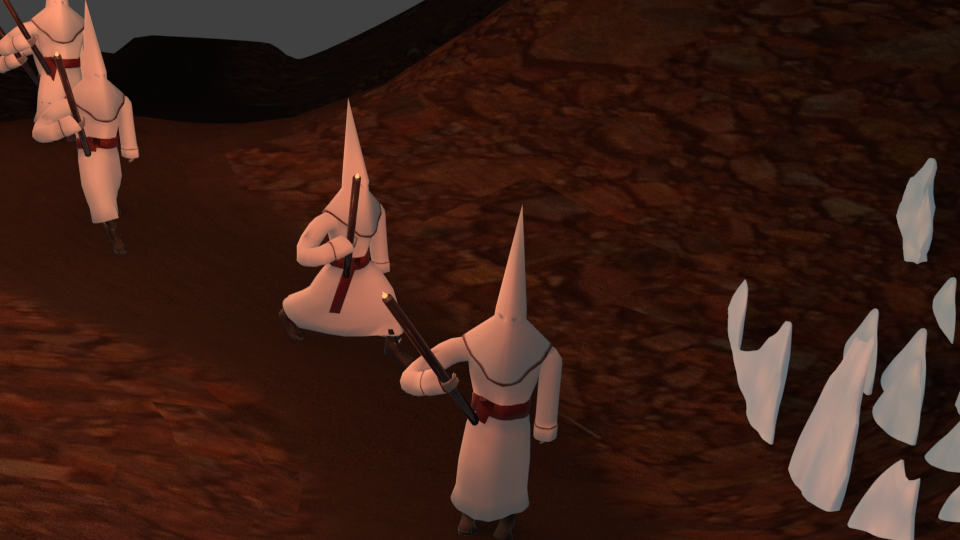
\includegraphics[height=5cm]{output.png}
	\end{center}
	\vfill
	\begin{center}
		\begin{large}
			\today\\
			\AuthorB & \url{\AuthorBEmail} \\
			\\
				& \Faculty \\
				& \School \\
		\end{large}
	\end{center}

\end{titlepage}		



% ----- obsah --------------------------------------------------------------

\tableofcontents

% ----- zadani -------------------------------------------------------------	
\newpage

\setlength{\parskip}{\baselineskip}
\setlength\parindent{0pt}

%---------------------------------------------------------------------------
\section{Introduction}
% V rámci tohoto projektu bude vytvořena scéna v Blenderu obsahující model sněhových kajícníků a animovaný průchod lidský kajícníků se svícemi. V rámci projektu budou použity modelovací nástroje, nástroje pro vytváření materiálů a texturu pomocí nodes a nástroje po skeletal animation. All project files are available at https://github.com/xchuki00/VIZa. 
As part of this project, a scene will be created in Blender containing a model of snow penitents and an animated passage of human penitents with candles. The project will use modeling tools, tools for creating materials and textures using nodes and tools for skeletal animation. All project files are available at https://github.com/xchuki00/VIZa. 
\section{Theoretical foundations}
\subsection{Subdivision modeling}
% Subdivision modeling je technika či způsob vytváření modelů ze základních tvarů, krychle či plocha, postupný dělení povrchu na menší a menší primitiva. Dělení může probíhat buď plošně, celý objekt, nebo jen lokálně. V Blenderu k tomu to postupu složí nástroje jako je \textit{knife}, \textit{loop cut} nebo \textit{subdivide}(každý čtverec povrchu objektu rozčtvrtí). Tento postup umožnuje nejdříve vymodelovat hrubé rysy a postupně zjemňovat. Výsledek tohoto modelování je možné převést na T-spline model.

Subdivision modeling\cite{sm} is a technique or method of creating models from basic shapes, cubes or~surfaces, gradual division of the surface into smaller and smaller primitives. The division can take place either flatly, the whole object, or only locally. In Blender, tools such as \textit{knife}, \textit{loop cut} or~\textit{subdivide} are used to do this (quarter each square of the object's surface). This procedure allows you to~first model the rough features and gradually refine. The result of this modeling can be converted to a T-spline model.

\subsection{T-splines}
% T-splines je metoda popisu povrchu podboná popisu pomocí NURBS křivek, jen nepotřebuje pravidelnou čtvercovou síť vrcholů. Metoda používá k popisu povrchu síť bodů a T-spline křivku, princip je dost podobný klasickému popisu povrchu jen místo spojování povrchu rovnými plochami, jsou body spojováný zakřivenými rovinami dle T-spline křivky. Teto reprezentace umožnujě vytvářet hladší a oblejší povrchy při minimálním navýšeni velikosti modelu. Lze díky tomu vytváře oblé a organické tvary, bez vysokého množství bodů. Tyto modely buď tvoříme na základe modelu vzniklého třeba Subdivision modeling nebo definováním křívky a jejím tažením/rotováním..., a následný spojováním takto vzniklých útvarů.     
T-splines is a surface description method similar to description using NURBS curves, it just doesn't need a regular square network of~vertices. The method uses a network of points and a T-spline curve to describe the surface, the principle is quite similar to~the~classical surface description only instead of~connecting the surface with flat surfaces, the points are connected by curved planes according to~the T-spline curve. This representation allows you to create smoother and rounder surfaces with minimal increase in model size. This makes it possible to create round and organic shapes without a~high number of points. We can create these models on the basis of a model created, for example, by~Subdivision modeling, or by defining a cross and dragging / rotating it ..., and then joining the~resulting shapes.
\subsection{Textures}
% Textura obecně definuje optické vlastnosti modelu. Může se jednat o jen obrázek namapovaný na model, nebo celou sadu "obrázků", definující optické vlastnosti jako hrubost, normály, odrazivost nebo třeba barvu. Díky nim model získává realistický vzhled, takže místo konstantní barvě a optických vlastnostech na celém objektu, můžou mít různá místa jinou odrazivost či barvu. V blenderu jsou textury zaobaleny Materiálem, který přiřazujeme objektu či jeho částem. Tento materiál je souhrnem několika typů textur, obsahuje barvu, hrubost, svítivost a tak dále. Pomocí Node editoru/Shader editoru se dá k každé vlastnosti, místo pevně nastavené hodnoty (Roughnest =0.5) připojit vstupní uzel, buď obrázek,generátor šumu či voronoidů a další. Každý objekt, který má mít textur musím vygenerovanou UV mapu, souřadný systém říkající, kde daný vertex leží na textuře. UV mapa tedy mapuje body 3D(většinou) tělesa na body 2D(většinou) textury. Textury nutně nemusí být 2D, mohou být jen 1D, tzn body tělas potom mapuji na přímku, nebo i N-D, potom se jedná o sadu 2D textur.      
The texture generally defines the optical properties of the model. It can be just an image mapped to~a~model, or a whole set of "images", defining optical properties such as roughness, normal, reflectivity or even color. Thanks to them, the model acquires a realistic appearance, so that instead of constant color and optical properties throughout the object, different places may have a different reflectivity or~color. In the blender, the textures are wrapped in the material we assign to the object or~its parts. This material is a collection of several types of textures, contains color, roughness, luminosity and so on. Using the Node editor / Shader editor, it is possible to connect an input node to each property, instead of a fixed value (Roughnest = 0.5), either an image, a noise generator or voronoids and more. For each object that is supposed to have a texture I need a generated UV map, a coordinate system telling where the vertex lies on the texture. The UV map therefore maps the points of a 3D (mostly) solid to the points of a 2D (mostly) texture. Textures do not necessarily have to be 2D, they can only be 1D, ie the body points are then mapped to a straight line, or even N-D, then it is a set of~2D textures.
\section{Motivation and goals}
% Motivací bylo vytvořit si komplexnější model pro diplomovou práci, jejíž zadání je Simulace a vizualizace Sněhu, konkrétně se zabývá volumetrickým vykreslování sněhových útvarů Kajícníků. A abych neprodával stejnou práci dvakrát rozhodl jsem se scénu rozšřit o průvod kajícníků, to jest průvod lidí konající pokání v zvláštním druhu pláště po nichž jsou ony sněhové útvary pojmenované. Dále mi motivací bylo se vyzkoušet co nejvíc funkcionality v Blenderu. 
The motivation was to create a more complex model for the diploma thesis, the assignment of thesis is Simulation and Visualization of Snow, specifically deals with the volumetric rendering of snow formations of Penitents. And in order not to sell the same work twice, I decided to expand the scene with a procession of penitents, that is, a procession of people repenting in a special kind of cloak after which the snow formations are named. Furthermore, my motivation was to try as much functionality as possible in Blender.

\section{Workflow description}
% Projekt jsem si rozdělil do několika úkolů: vytvořit terén (úbočí a cestu), nainstalovaní modelů kajícníků (sněhových útvarů) na úbočí hory, vytvoření modelu lidského kajícníka a následné naanimování scény.
I divided the project into several tasks: creating the terrain (hillside and path), installing models of penitents (snow formations) on the mountainside, creating a model of a human penitent and then animating the scene.
\subsection{Terrain}
% Terén jsem modeloval z plochy, tuto plochu jsem nejdříve jen lehce rozdělil a zvrásnil pohybem vektorů se zapnutým \textit{Proportional editing obejct}, na následně \textit{sculp mode} dotvaroval a vyzdvihl násep cesty. V případě tohoto modelu jsem mnohem více času než s modelováním strávil se snahou vytvořit věrohodnou texturu. Původně jsem zkoušel kombinovat v \textit{Shader editoru} dvě nodes \textit{Principel BSDF}, každé nastavil základní a podkladovou barvu, následně použil šum k určení poměru prosvítání podkladové barvy a míchání mezi oběma nodes, ale výsledek nebyl příliš kvalitní, nakonec jsem uchýlil k textuře na základě fotky stažené z pixbay  a tuto fotku použil jako barevný vstup pro jednu z \textit{Principel BSDF} node. Dále jsem na základě jedné šumové funkce upravoval normály a hrubost textur.  
I modeled the terrain from the surface, at first I only slightly divided this surface and wrinkled it by moving vectors with \textit{Proportional editing obejct} turned on, then on \textit{sculp mode} crept up and lifted the road embankment. In the case of this model, I spent much more time than modeling trying to create a believable texture. I originally tried to combine two nodes \textit{Principel BSDF} in the \textit{Shader editor}, each set the base and background colors, then used the noise to determine the ratio of translucency of the background color and mixing between the two nodes, but the result was not very good, he resorted to texture based on a photo downloaded from pixbay and used that photo as color input for one of the \textit{Principel BSDF} node. I also adjusted the normals and roughness of the textures based on one noise function.
\begin {center}
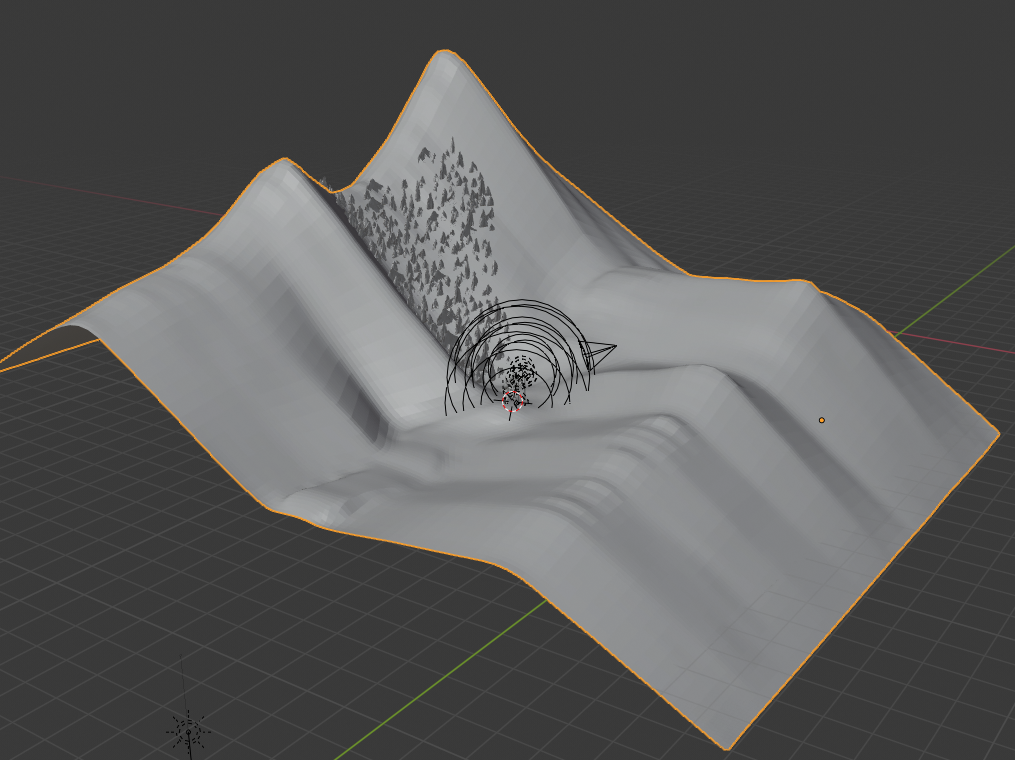
\includegraphics [height = 10cm] {terrain.png}
% \caption {Terén s kajícníkem a kajícníky(sněhovými útvary)}
\caption {Terrain with penitent and penitents (snow formations)}
\end {center}
\subsection{Snow formation Penitents}
% Jedná se asi o dvacet různých modelů vytvořených v rámci mé diplomové práce, pro účely toho projektu jsem je rozmístil na úbočí, vzhledem k vysoké proměnlivosti a nahodilosti terénu bylo třeba umístit ručně každý útvar. Původních dvacet modelů jsem z duplikoval a vytvořil tak menší kajícníkové pole asi o 160 útvarech. Dále jsou doplněny o materiál se základní bílou barvou, trochou světlounce modrého vyzařování a voronový diagramem určený prosvítáním světle modré barvy. 
These are about twenty different models created within my diploma thesis, for the purposes of this project I placed them on the hillside, due to the high variability and randomness of the terrain, it was necessary to place each department by hand. I duplicated the original twenty models and created a smaller penitent field of about 160 formations. They are also supplemented by a material with a basic white color, a little light blue light and a voron diagram determined by the light blue translucency.
\subsection{Model of Penitent(human)}
% Pro inspiraci tvaru a vzhledu postav a tedy i jejich oděvu mi sloužila fotografie z pinterestu\footnote{https://www.pinterest.es/pin/419116309057507217/}. A to vzhledem ke specifičnosti hábitu, který nosí. Jak bylo výše zmíněno, tento oděv je inspirovaný právě mnou modelovanými kajícníky.
% 		\begin{center}
% 		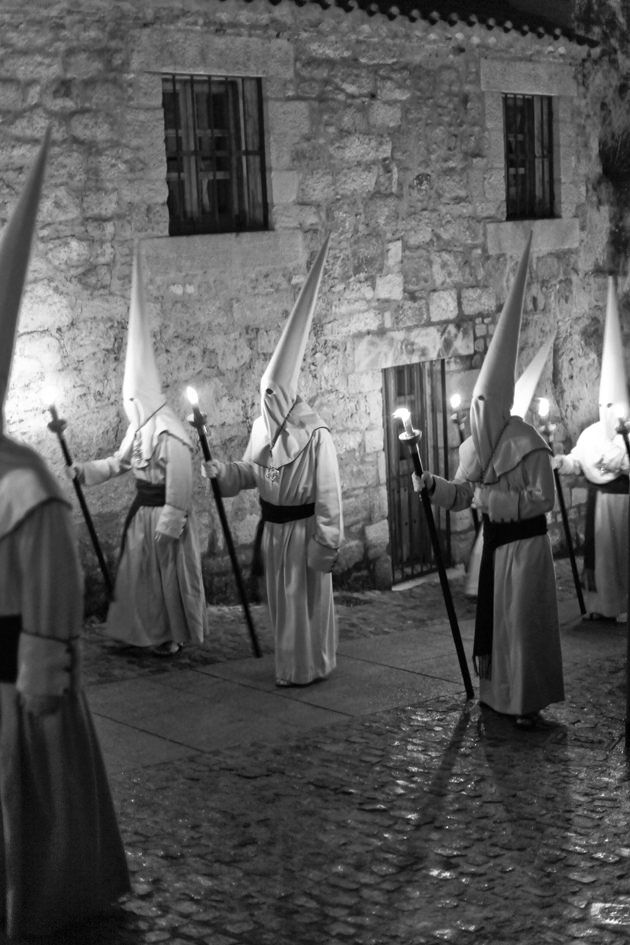
\includegraphics[height=10cm]{předloha.jpg}
% 		\caption{https://www.pinterest.es/pin/419116309057507217/}
% 	\end{center}
% Jinak je tento model celý vytvářený v Blenderu, pomocí subdivision modelingu z válců (tělo, svíce), samostatně jsou tvořeny dlaně (krychle) a nohy (plane). Následně byla modelu dotvořena kostra s automatickým rozdělením vah, které muselo být v oblasti chodidel upraveno. Neboť docházelo k ovlivňování obou chodidel kostmi jednoho chodidla tzn. že při pohybu levého kotníku mi docházelo k nesouměrnému hýbání pravého i levého chodidla zároveň. Plus musela být dotvořena samozřejmě textura. V tomto případě celá ručně malovaná, jedná se o bílou plocha s vínovým lemováním, šerpou a několika detaily. Svíce nemá bohužel důkladně vymodelovaný plamen, jen statický, ale vzhledem k velikosti scény není bohužel příliš vidět. Tedy jsem naznal, že není potřeba se s plamenem důkladněji modelovat než jen pro samotný nástin, jeho existence. Plamen má materiál s nastaveným vyzařováním v oranžové barvě a následně jsou k němu připojeny tři bodové zdroje světla o různých odstínech žluté až oranžové a s různou intenzitou a dosahem (čím tmavší světlo tím menší dosah) pro vytvoveření iluze pravého plamene.
To inspire the shape and appearance of the characters and therefore their clothing, I used a photo from pinterest \footnote {https://www.pinterest.es/pin/419116309057507217/}. This is due to the specificity of the robe he wears. As mentioned above, this garment is inspired by the penitents I modeled.
\begin {center}
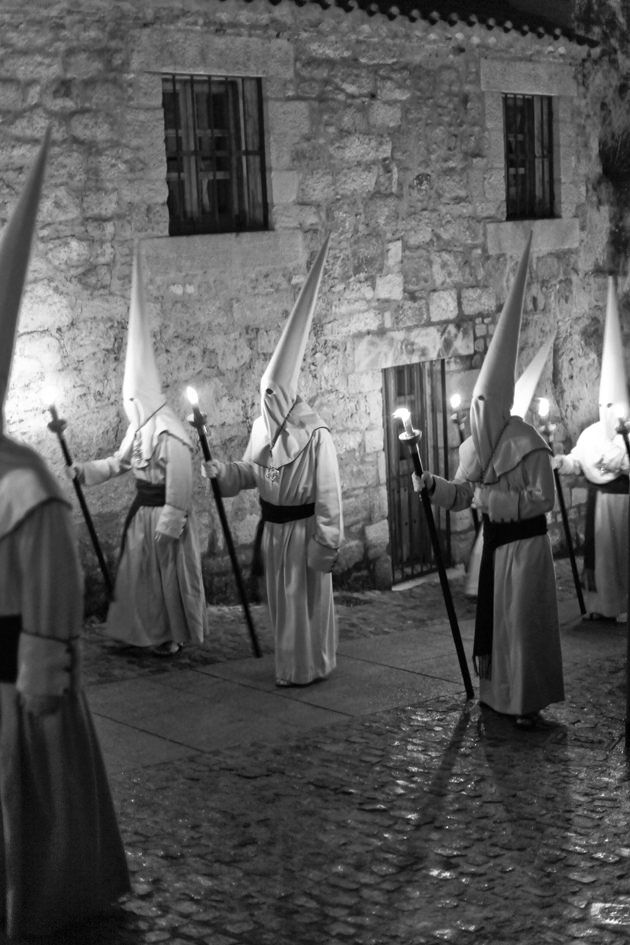
\includegraphics [height = 10cm] {předloha.jpg}
\caption {https://www.pinterest.es/pin/419116309057507217/}
\end {center}
Otherwise, this whole model is created in Blender, using subdivision modeling from cylinders (body, candle), palms and legs are formed separately. Subsequently, the model was completed with a skeleton with automatic weight distribution, which had to be adjusted in the area of ​​the feet. Because both feet were affected by the bones of one foot, ie. that while moving my left ankle, my right and left foot moved asymmetrically at the same time. Plus, of course, the texture had to be completed. In this case, the whole hand-painted, it is a white surface with burgundy edging, sash and a few details. Unfortunately, the candle does not have a thoroughly modeled flame, only static, but unfortunately it is not very visible due to the size of the scene. So I realized that there is no need to model the flame more thoroughly than just for the outline itself, its existence. The flame has a material with a set emission in orange, and then three point light sources of different shades of yellow to orange and with different intensity and range (the darker the light the smaller the range) are connected to it to create the illusion of a true flame.
\begin {center}
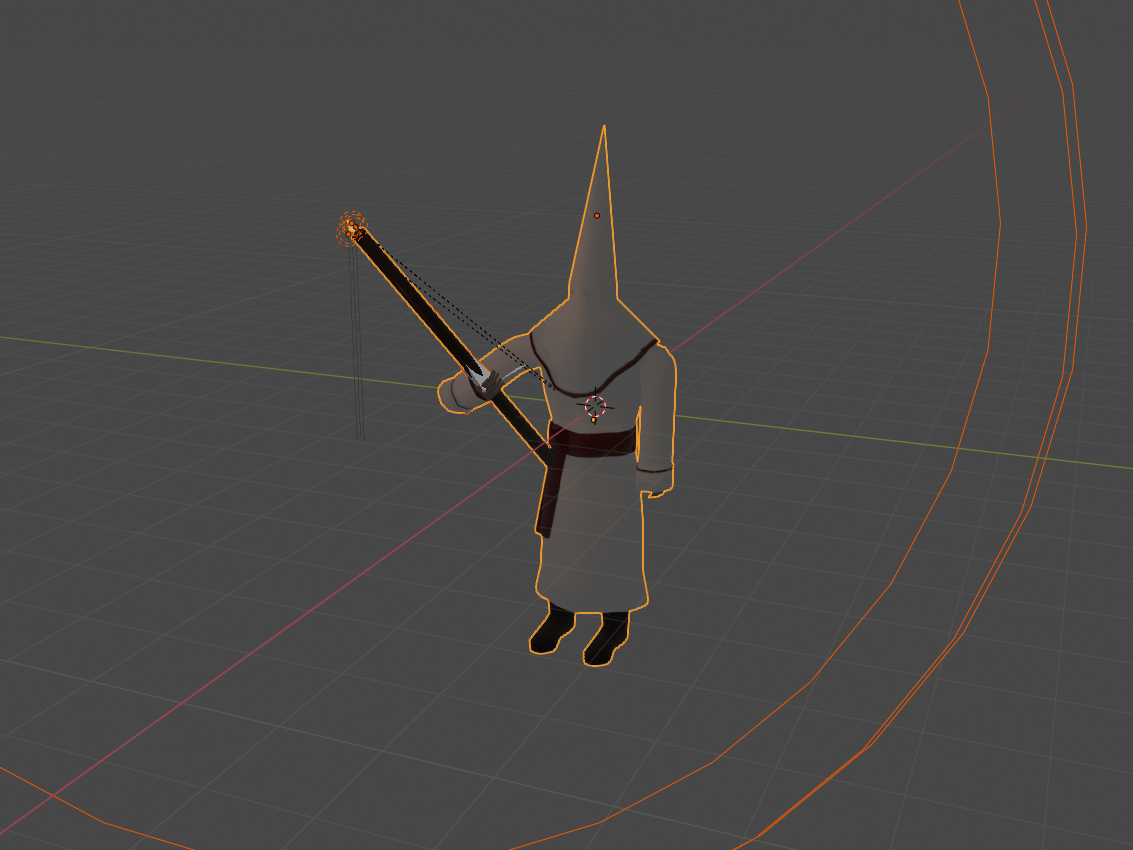
\includegraphics [height = 10cm] {PenitenteModel.png}
% \caption {Model kajícníka}
\caption {Model of a penitent}
\end {center}
\subsection{Animating}
% Animace je tvořena pomocí kostry Kajícníka, největší problémem byla délka kroku postavy. Protože při chůzi z kopce, do kopce či po rovince se jeho délka a sklon mění. Z tohoto důvodu musel být každý krok modelován zvlášť. K usnadnění jsem si vytvořil třetí texturu pro terén. Na ní jsem si vyznačil otisky nohou, abych věděl kam má které noha došlápnout a odkud se která noha odráží. Všech pět kajícníků kteří se ve výsledné animaci ukáží, jsou tedy kopie toho prvního, pouze s posunutým časováním.
The animation is created using the Penitent of the Penitent, the biggest problem was the length of the character's step. Because when walking downhill, uphill or on a straight line, its length and inclination change. For this reason, each step had to be modeled separately. To make it easier, I created a third texture for the terrain. I marked my footprints on it to know where each foot should step on and where each foot bounces off. All five penitents who appear in the resulting animation are therefore copies of the first, only with a shifted timing.

\section{Results}
% Výsledkem projektu je scéna v Blendru obsahující skeletal animation a modely kajícníků. Včetně naanimovaného pohybu kamery. Hlavním výstupem je tedy vykreslené video na němž je možné vidět průvod kajícníků s velkými voskovice po cestě pod zformovanými kajícníky. Všechy soubory projektu jsou k dispozici na adrese https://github.com/xchuki00/VIZa.
The result of the project is a scene in Blender containing skeletal animation and models of penitents. Including animated camera movement. The main output is therefore a video rendered in which it is possible to see a procession of penitents with large candle on the way under the formed penitents. All project files are available at https://github.com/xchuki00/VIZa.
\section{Conclusion}
% Výsledný product není špatný, avšak bylo by potřeba  zdokonalit texturu hor a animaci chůze Kajícníků. To se mi bohužel z nedostatku času nepodařilo tak, jak bych sám chtěl. Na druhou stranu celkový výsledek obsahuje několik použitých technik: nodes, sculpt tools, jednoduché osvětlení animované v čase a skeleton animation pro pohyb Kajícníků. Čímž jsem splnil svou vlastní motivaci vyzkoušet si co nejvíce funkcí Blenderu, jak jen to půjde. Celkově jsem se mnohé naučil, každá část z výsledné animace by mohla být dokonalejší, to by však při velikosti scény bylo pro tento menší projekt možná až zbytečné obsáhlé. Téma a možnosti animaci by však mohli pro někoho obsáhnout i bakalářskou práci.     
The resulting product is not bad, but it would like to improve the texture of the mountains and the animation of the walking of the Penitents. But overall, the result includes several techniques used, nodes, sculpt tools, simple lighting animated in time and skeleton animation for the movement of the Penitents. Overall, I learned a lot, each part could be more perfect, but then with this complexity of the scene, it might be a little bachelor thesis.
\newpage
\section{List of  figures}
\begin {center}
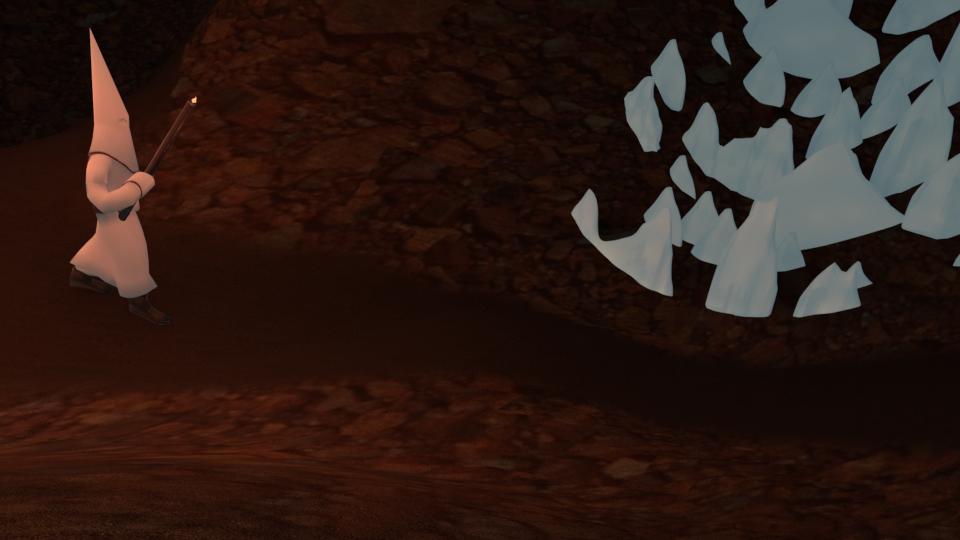
\includegraphics [height = 10cm] {FirstPenitente.png}
% \caption {Model kajícníka}
\caption {Model of a penitent}
\end {center}
\begin {center}
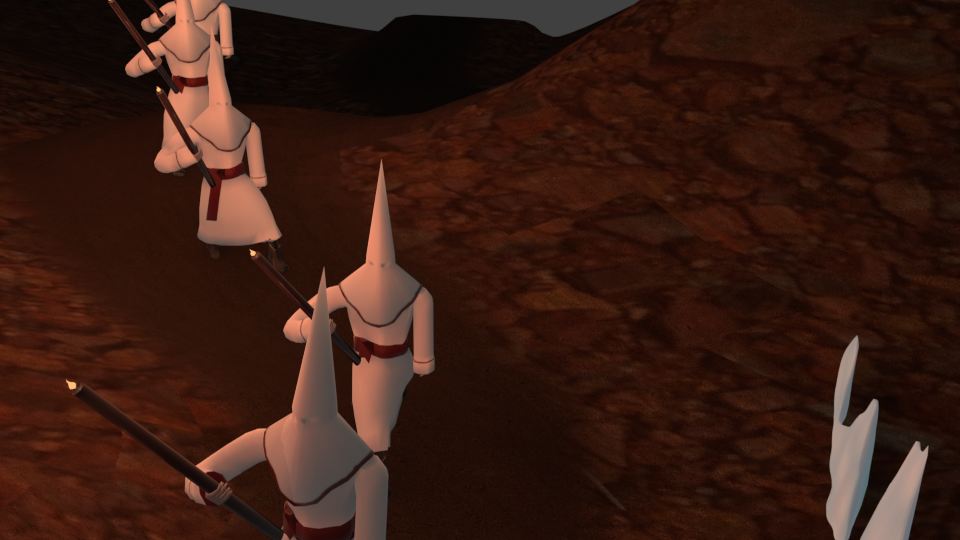
\includegraphics [height = 10cm] {procession.png}
% \caption {Model kajícníka}
\caption {Model of a penitent}
\end {center}
\begin {center}
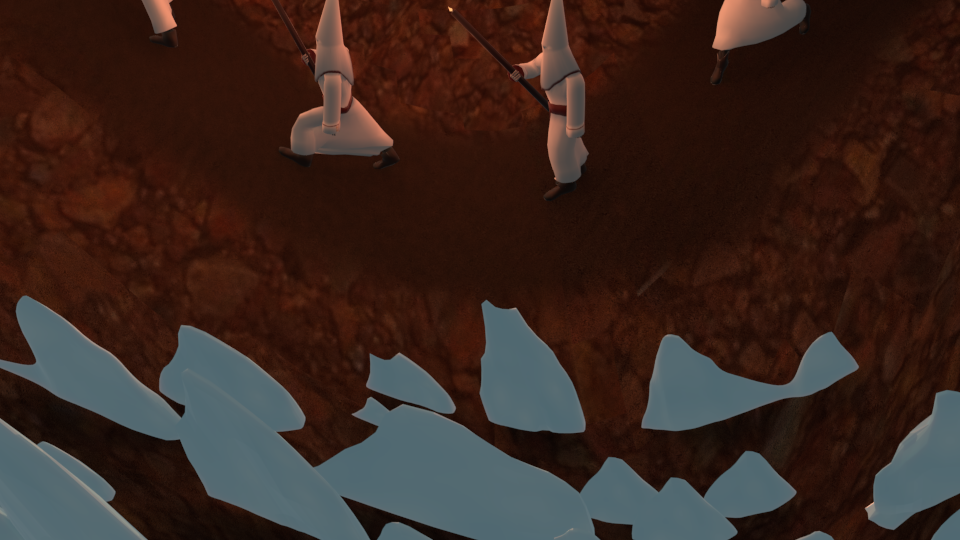
\includegraphics [height = 10cm] {PenitenteAndPenitentes.png}
% \caption {Model kajícníka}
\caption {Model of a penitent}
\end {center}
\begin {center}
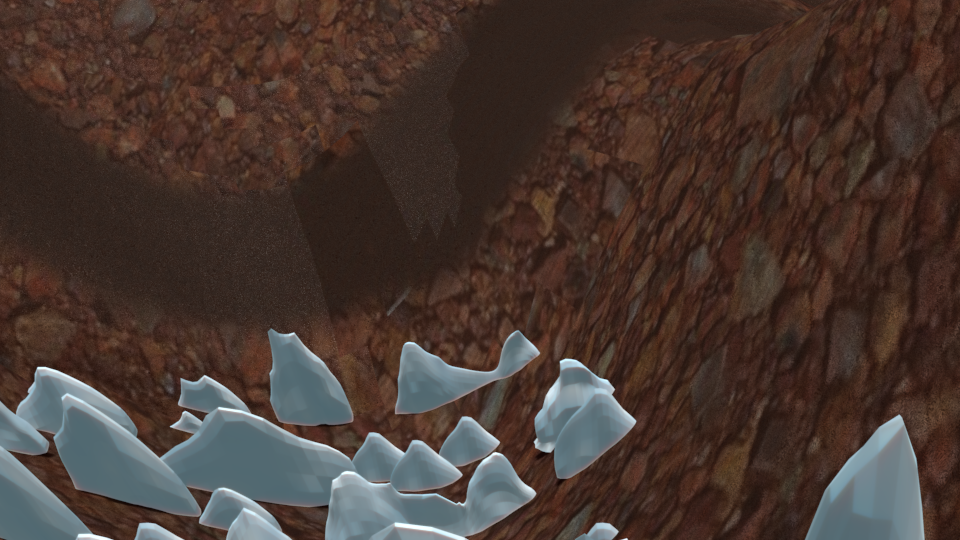
\includegraphics [height = 10cm] {Penitentes.png}
% \caption {Model kajícníka}
\caption {Model of a penitent}
\end {center}
% %---------------------------------------------------------------------------

 \bibliographystyle{enplain}

\bibliography{reference}
\addcontentsline{toc}{section}{Literature}

\end{document}

